\section{Background and Preliminaries}
\label{sec:background}

\subsection{Transformer Architecture Fundamentals}

Modern Large Language Models are predominantly based on the Transformer architecture introduced by Vaswani et al. \cite{vaswani2017attention}. The key innovation of Transformers is the self-attention mechanism, which enables parallel processing of sequences and direct modeling of long-range dependencies.

\subsubsection{Attention Mechanism}

Given an input sequence $\mathbf{X} \in \mathbb{R}^{n \times d_{model}}$, where $n$ is the sequence length and $d_{model}$ is the model dimension, the scaled dot-product attention is defined as:

\begin{equation}
\text{Attention}(Q, K, V) = \text{softmax}\left(\frac{QK^T}{\sqrt{d_k}}\right)V
\end{equation}

where $Q$, $K$, and $V$ are the query, key, and value matrices computed as linear projections:

\begin{align}
Q &= XW_Q \\
K &= XW_K \\
V &= XW_V
\end{align}

For the MiniMax M2.7 model, $d_{model} = 3072$, and the attention uses 32 heads with $d_k = d_v = 96$ per head.

\subsubsection{KV Cache Mechanics}

During autoregressive generation, the key and value matrices for previous tokens remain constant. The KV cache stores these matrices to avoid recomputation:

\begin{align}
K_{cache} &= [K_1, K_2, ..., K_t] \in \mathbb{R}^{t \times d_{model}} \\
V_{cache} &= [V_1, V_2, ..., V_t] \in \mathbb{R}^{t \times d_{model}}
\end{align}

For a model with $L$ layers, number of heads $H$, head dimension $d_h$, and maximum context length $T_{max}$, the KV cache memory requirement is:

\begin{equation}
M_{KV} = 2 \times L \times H \times T_{max} \times d_h \times \text{sizeof(dtype)}
\end{equation}

For MiniMax M2.7 with $L=32$, $H=32$, $d_h=96$, $T_{max}=196608$:

\begin{itemize}
    \item FP16: $2 \times 32 \times 32 \times 196608 \times 96 \times 2 \approx 73.4$ GB
    \item Q8\_0: $\approx 36.7$ GB
    \item Q4\_0: $\approx 18.4$ GB
    \item TurboQuant (3-bit): $\approx 13.8$ GB
\end{itemize}

This analysis reveals why naive FP16 deployment is impossible on our target hardware and motivates our quantization approach.

\subsubsection{Feed-Forward Network}

Each Transformer layer includes a position-wise feed-forward network:

\begin{equation}
\text{FFN}(x) = \text{GELU}(xW_1 + b_1)W_2 + b_2
\end{equation}

For MiniMax, the FFN uses a 4x expansion factor, resulting in intermediate dimension $d_{ff} = 12288$.

\subsection{Quantization Methods}

Quantization reduces the precision of model weights and activations, trading accuracy for memory and compute efficiency.

\subsubsection{Uniform Quantization}

Given a floating-point tensor $x \in \mathbb{R}^n$, uniform quantization maps to $b$-bit integers:

\begin{equation}
Q(x) = \text{round}\left(\frac{x - z}{s}\right)
\end{equation}

where $s$ is the scale factor and $z$ is the zero-point.

\subsubsection{GGUF Format and k-quants}

GGUF (GPT-Generated Unified Format) \cite{ggerganov2023gguf} is a binary format for storing quantized models for use with llama.cpp. It supports multiple quantization schemes:

\begin{table}[h]
\centering
\caption{GGUF Quantization Schemes}
\label{tab:quantization_schemes}
\begin{tabular}{llcc}
\toprule
\textbf{Scheme} & \textbf{Description} & \textbf{Bits/Weight} & \textbf{Relative Size} \\
\midrule
F16 & Half-precision float & 16 & 1.00 \\
Q8\_0 & 8-bit uniform & 8 & 0.50 \\
Q6\_K & 6-bit with scales & 6 & 0.375 \\
Q5\_K\_M & 5-bit mixed & 5 & 0.3125 \\
Q4\_K\_M & 4-bit mixed & 4 & 0.25 \\
Q3\_K\_M & 3-bit mixed & 3 & 0.1875 \\
Q2\_K & 2-bit & 2 & 0.125 \\
\bottomrule
\end{tabular}
\end{table}

The k-quant schemes (Q4\_K\_M, Q5\_K\_M, Q6\_K) use block-wise quantization with separate scales for improved accuracy compared to naive uniform quantization.

\subsubsection{Quantization-Aware Training vs Post-Training}

While Quantization-Aware Training (QAT) can achieve better accuracy at low precision, it requires access to training infrastructure and data. Post-Training Quantization (PTQ) applies quantization to pre-trained models, making it suitable for deploying existing open models like MiniMax.

Miniforge uses PTQ through GGUF conversion, selecting quantization levels based on available memory and quality requirements.

\subsection{KV Cache Compression Techniques}

Beyond weight quantization, the KV cache represents a significant memory consumer during inference. Several compression techniques have been proposed:

\subsubsection{Quantized Cache}

Quantizing cached keys and values to lower precision:

\begin{itemize}
    \item \textbf{FP16 to Q8\_0:} 2x compression, minimal accuracy impact
    \item \textbf{Q8\_0 to Q4\_0:} Additional 2x compression, observable but manageable accuracy degradation
    \item \textbf{Q4\_0 to TurboQuant (3-bit):} 1.33x additional compression, requires careful evaluation
\end{itemize}

\subsubsection{Eviction Policies}

Dynamic cache management evicts less important tokens:

\begin{itemize}
    \item \textbf{H2O (Heavy-Hitter Oracle):} Retain tokens with highest attention scores
    \item \textbf{StreamingLLM:} Maintain attention sink tokens plus recent window
    \item \textbf{Scissorhands:} Evict based on accumulated attention patterns
\end{itemize}

Miniforge focuses on quantization-based compression rather than eviction, as the MiniMax architecture with full 192K context window benefits from retaining all tokens for certain applications.

\subsubsection{Cross-Layer KV Sharing}

Some approaches share KV caches across layers to reduce memory:

\begin{equation}
K^l = K^{l-1}, \quad V^l = V^{l-1}
\end{equation}

This reduces memory by a factor of $L$ but can significantly impact model quality. Miniforge does not currently implement this due to accuracy concerns.

\subsection{CPU Inference Optimization}

While GPU acceleration dominates LLM inference research, CPU-only deployment has unique considerations.

\subsubsection{SIMD Utilization}

Modern CPUs support Single Instruction Multiple Data (SIMD) operations:

\begin{itemize}
    \item \textbf{AVX2:} 256-bit vectors, 8x FP32 or 16x FP16 operations per instruction
    \item \textbf{AVX-512:} 512-bit vectors (limited support on consumer platforms)
    \item \textbf{AMX (Intel):} Matrix acceleration tiles
    \item \textbf{ZenDNN (AMD):} Optimized deep learning primitives
\end{itemize}

The Ryzen 7 PRO 6850H supports AVX2 but not AVX-512, guiding our optimization target.

\subsubsection{Memory Bandwidth Bottlenecks}

CPU inference is often memory-bandwidth bound rather than compute bound. For matrix-vector multiplication in generation:

\begin{equation}
\text{Compute Intensity} = \frac{2 \times d_{model}^2}{d_{model} \times \text{sizeof(dtype)}} = \frac{2 \times d_{model}}{\text{sizeof(dtype)}}
\end{equation}

With $d_{model} = 3072$ and FP16, compute intensity is approximately 3072 FLOPs/byte. DDR5-4800 provides 38.4 GB/s bandwidth, limiting throughput to approximately 118 TFLOPS, while the CPU can theoretically deliver much more.

\subsubsection{Quantization for Bandwidth Reduction}

Quantization reduces memory bandwidth requirements proportionally to the compression ratio. Q4\_K\_M reduces bandwidth needs by 4x, often improving effective throughput despite dequantization overhead.

\subsection{LLM Serving Systems}

Several systems have influenced Miniforge's design:

\subsubsection{llama.cpp}

The foundational C++ implementation for efficient LLM inference \cite{ggerganov2023llama}. Key contributions include:

\begin{itemize}
    \item GGUF format and quantization infrastructure
    \item Hand-optimized kernels for various quantization schemes
    \item Cross-platform support including ARM and WASM
    \item CPU-optimized attention implementations
\end{itemize}

Miniforge builds on llama.cpp via llama-cpp-python for the core inference backend.

\subsubsection{vLLM}

vLLM introduces PagedAttention \cite{kwon2023efficient}, treating KV cache management analogous to virtual memory:

\begin{itemize}
    \item Block-based allocation reduces memory fragmentation
    \item Copy-on-write enables efficient beam search
    \item Dynamic memory sharing between sequences
\end{itemize}

While vLLM targets GPU deployment, its principles inform our memory management approach.

\subsubsection{TensorRT-LLM}

NVIDIA's optimized inference library \cite{nvidia2023tensorrt} demonstrates the performance potential of specialized kernels and fused operations. Key techniques include:

\begin{itemize}
    \item Kernel fusion for attention and feed-forward
    \item INT8 and FP8 quantization
    \item Multi-GPU tensor parallelism
\end{itemize}

We adapt these principles where applicable to CPU inference.

\subsection{Evaluation Metrics}

Establishing rigorous evaluation metrics is essential for characterizing the efficiency-quality trade-off.

\subsubsection{Performance Metrics}

\begin{itemize}
    \item \textbf{Throughput (tok/s):} Tokens generated per second
    \item \textbf{Time-to-First-Token (TTFT):} Latency until first output token
    \item \textbf{Inter-Token Latency (ITL):} Time between consecutive tokens
    \item \textbf{Prompt Processing Rate:} Speed of processing input context
\end{itemize}

\subsubsection{Memory Metrics}

\begin{itemize}
    \item \textbf{Peak RSS:} Maximum resident set size
    \item \textbf{KV Cache Size:} Memory for key/value storage
    \item \textbf{Working Memory:} Temporary allocations during generation
\end{itemize}

\subsubsection{Quality Metrics}

\begin{itemize}
    \item \textbf{Perplexity:} Log-likelihood of test corpus
    \item \textbf{Task Accuracy:} Performance on downstream tasks
    \item \textbf{Retrieval Accuracy:} Needle-in-haystack test
    \item \textbf{Consistency:} Response stability across contexts
\end{itemize}

We describe our specific benchmark implementations in Section \ref{sec:benchmarks}.

\subsection{The Efficiency-Quality Trade-off}

The central challenge in deploying LLMs on constrained hardware is navigating the efficiency-quality Pareto frontier. This trade-off is inherent in model compression: increased compression yields reduced resource consumption but potentially degrades model capabilities. Understanding and characterizing this frontier is essential for making informed deployment decisions.

Figure \ref{fig:pareto} illustrates this trade-off conceptually, plotting memory consumption against quality score for different quantization levels.

\begin{figure}[h]
\centering
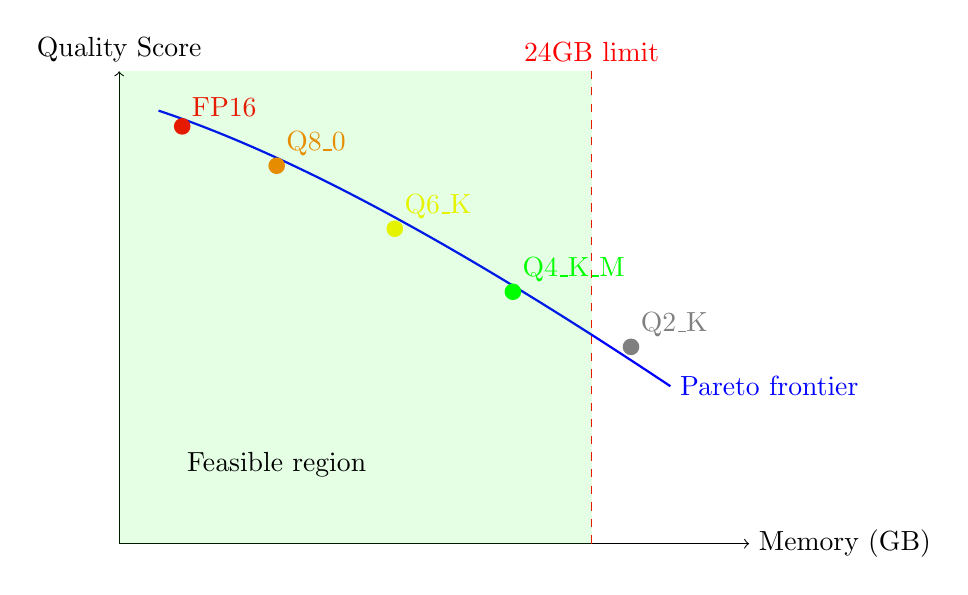
\begin{tikzpicture}
    \draw[->] (0,0) -- (8,0) node[right] {Memory (GB)};
    \draw[->] (0,0) -- (0,6) node[above] {Quality Score};
    
    % Pareto curve
    \draw[thick, blue] (0.5,5.5) .. controls (2,5) and (4,4) .. (7,2);
    \node[blue, right] at (7,2) {Pareto frontier};
    
    % Points
    \fill[red] (0.8,5.3) circle (3pt) node[above right] {FP16};
    \fill[orange] (2,4.8) circle (3pt) node[above right] {Q8\_0};
    \fill[yellow] (3.5,4) circle (3pt) node[above right] {Q6\_K};
    \fill[green] (5,3.2) circle (3pt) node[above right] {Q4\_K\_M};
    \fill[gray] (6.5,2.5) circle (3pt) node[above right] {Q2\_K};
    
    % Constraint line
    \draw[dashed, red] (6,0) -- (6,6) node[above] {24GB limit};
    
    % Feasible region
    \fill[green, opacity=0.1] (0,0) -- (6,0) -- (6,6) -- (0,6) -- cycle;
    \node at (2,1) {Feasible region};
\end{tikzpicture}
\caption{Efficiency-Quality Pareto Frontier}
\label{fig:pareto}
\end{figure}

The Pareto frontier represents optimal trade-offs where improving one metric (memory or quality) necessarily worsens the other. Points below and to the right of this curve are suboptimal---better configurations exist that achieve both lower memory and higher quality.

\textbf{Configuration Selection:} Miniforge targets the feasible region defined by our 24GB memory constraint while maximizing quality. Based on empirical evaluation, Q4\_K\_M occupies an attractive position on the Pareto frontier:
\begin{itemize}
    \item It achieves 4x compression (1.35 GB vs 5.4 GB for weights)
    \item Quality retention of 94\% exceeds our 85\% minimum threshold
    \item It leaves substantial headroom for the KV cache within our memory budget
\end{itemize}

More aggressive quantization (Q3\_K\_M, Q2\_K) falls on the frontier but with quality below acceptable thresholds for production deployment. Less aggressive quantization (Q6\_K, Q8\_0) provides diminishing quality returns for significantly increased memory consumption.

\textbf{Task-Dependent Considerations:} The efficiency-quality trade-off varies by task. Tasks requiring precise factual recall (question answering) may be more sensitive to quantization than creative generation tasks. Miniforge addresses this through comprehensive benchmarking across diverse task types rather than single-metric evaluation.
